\paragraph[QuizziPedia::Front-End::Controllers\\::QuestionnaireDetailsController]{QuizziPedia::Front-End::Controllers::QuestionnaireDetailsController}
\begin{figure} [ht]
	\centering
	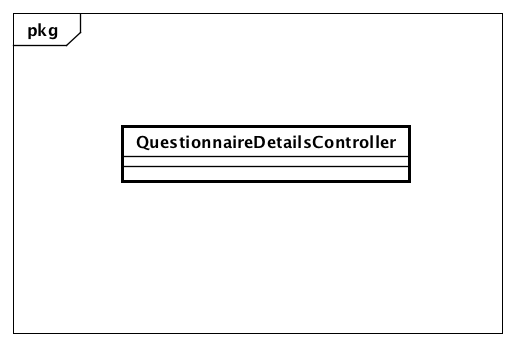
\includegraphics[scale=0.5]{UML/Classi/Front-End/QuizziPedia_Front-end_Controller_QuestionnaireDetailsController.png}
	\caption{QuizziPedia::Front-End::Controllers::QuestionnaireDetailsController}
\end{figure} \FloatBarrier
\begin{itemize}
	\item \textbf{Descrizione}: questa classe permette di gestire i dettagli di un questionario; 
	\item \textbf{Utilizzo}: fornisce le funzionalità per recuperare dal back-end i dettagli di un questionario creato da un utente al fine di poterli visualizzare nel suo profilo;
	\item \textbf{Relazione con altre classi}:
	\begin{itemize}
		\item \textbf{IN \texttt{QuestionnaireDetailsModelView}}: classe di tipo \textit{modelview\ped{G}} la cui istanziazione è contenuta all'interno della variabile di ambiente \$scope di \textit{Angular\ped{G}}. All'interno di essa sono presenti le variabili e i metodi necessari per il \textit{Two-Way Data-Binding\ped{G}} tra la \textit{view\ped{G}} \texttt{UserView} e il \textit{controller\ped{G}} \texttt{QuestionnaireDetailsController};
		\item \textbf{IN \texttt{QuizService}}: questa classe permette di ottenere i dati di un quiz tramite delle parole chiave inserite dall'utente nella barra di ricerca;
		\item \textbf{IN \texttt{QuestionnaireModel}}: rappresenta un questionario. Contiene tutte le informazioni necessarie alla presentazione del contenuto del questionario.
	\end{itemize}
	\item \textbf{Attributi}:
	\begin{itemize}
		\item \texttt{-} \texttt{\$scope: \$scope} \\
		Campo dati contenente un riferimento all'oggetto \$scope creato da \textit{Angular\ped{G}}, viene utilizzato come mezzo di comunicazione tra il \textit{controller\ped{G}} e la \textit{view\ped{G}}. Contiene gli oggetti che definiscono il \textit{model\ped{G}} dell'applicazione;
		\item \texttt{-} \texttt{\$rootScope: \$rootScope} \\
		Campo dati contenente il riferimento all'oggetto globale \$rootScope creato da \textit{Angular\ped{G}}. Viene utilizzato per rendere accessibile a tutti i \textit{controller\ped{G}} e a tutte le \textit{view\ped{G}} l'oggetto \texttt{QuestionnaireModel}. In questo caso viene utilizzato per inserire in \$rootScope l'oggetto di ritorno della chiamata a \texttt{getQuestionnaireDetails} del \textit{service\ped{G}} \texttt{QuizService};
		\item \texttt{-} \texttt{QuizService: QuizService} \\ Questa classe permette di ottenere i dati di un quiz tramite delle parole chiave inserite dall'utente nella barra di ricerca;
		\item \texttt{-} \texttt{\$mdDialog: \$mdDialog} \\
		Parametro contenente un riferimento al servizio della libreria \textit{Material for Angular\ped{G}} che permette di creare delle componenti a pop-up;
		\item \texttt{+} \texttt{details: QuestionnaireDetailsModelView} \\
		Oggetto di tipo \texttt{QuestionnaireDetailsModelView}. All'interno di esso sono presenti le variabili e i metodi necessari per il \textit{Two-Way Data-Binding\ped{G}} tra la \textit{view\ped{G}} \texttt{UserView} e il \textit{controller\ped{G}} \texttt{QuestionnaireDetailsController}.
	\end{itemize}
	\item \textbf{Metodi}:
	\begin{itemize}
		\item \texttt{+} \texttt{QuestionnaireDetailsController(\$scope: \$scope, \$rootScope: \$rootSc-\\ope, \$mdDialog: \$mdDialog, QuizService: QuizService)} \\ Metodo costruttore della classe. \\
		\textbf{Parametri}: 
		\begin{itemize}
			\item \texttt{\$scope: \$scope} \\
			Parametro contenente un riferimento all'oggetto \$scope creato da \textit{Angular\ped{G}}. Viene utilizzato come mezzo di comunicazione tra il \textit{controller\ped{G}} e la \textit{view\ped{G}}. Contiene gli oggetti che definiscono il \textit{viewmodel\ped{G}} e il \textit{model\ped{G}} dell'applicazione;
			\item \texttt{\$rootScope: \$rootScope} \\
			Parametro contenente il riferimento all'oggetto globale \$rootScope creato da \textit{Ang-\\ular\ped{G}}. Viene utilizzato per rendere accessibile a tutti i \textit{controller\ped{G}} e a tutte le \textit{view\ped{G}} l'oggetto \texttt{QuestionnaireModel}. In questo caso viene utilizzato per inserire in \$rootScope l'oggetto di ritorno della chiamata a \texttt{getQuestionnaireDetails} del \textit{service\ped{G}} \texttt{QuizService};	
			\item \texttt{\$mdDialog: \$mdDialog} \\
			Parametro contenente un riferimento al servizio della libreria \textit{Material for Angular\ped{G}} che permette di creare delle componenti a pop-up;
			\item \texttt{QuizService: QuizService}\\ Parametro che permette di ottenere, tramite il \textit{service\ped{G}}, la lista di tutte le domande presenti nel quiz.
		\end{itemize}
		
		\item \texttt{-} \texttt{getQuestionnaireDetails(username: String): Object} \\ Metodo che richiede al \textit{service\ped{G}} i dettagli dei questionari eseguiti dall'utente. \\
		\textbf{Parametri}:
		\begin{itemize}
			\item \texttt{username: String}: username dell'utente del quale caricare i questionari.
		\end{itemize}
		\item \texttt{-} \texttt{getSubscribedQuestionnaire(username: String): Object} \\Metodo che ritorna i questionari a cui l'utente è iscritto. \\
		\textbf{Parametri}:
		\begin{itemize}
			\item \texttt{username: String}: username dell'utente del quale scaricare i questionari a cui è iscritto.
		\end{itemize}
	\end{itemize}
\end{itemize}

